%==========================================
%
% Sibgrapi 2015 paper
%
%==========================================


% Note that the a4paper option is mainly intended so that authors in
% countries using A4 can easily print to A4 and see how their papers will
% look in print - the typesetting of the document will not typically be
% affected with changes in paper size (but the bottom and side margins will).
% Use the testflow package mentioned above to verify correct handling of
% both paper sizes by the user's LaTeX system.
%
% Also note that the "draftcls" or "draftclsnofoot", not "draft", option
% should be used if it is desired that the figures are to be displayed in
% draft mode.
%
\documentclass[10pt, conference]{IEEEtran}

% *** MISC UTILITY PACKAGES ***
%
%\usepackage{ifpdf}
% Heiko Oberdiek's ifpdf.sty is very useful if you need conditional
% compilation based on whether the output is pdf or dvi.
% usage:
% \ifpdf
%   % pdf code
% \else
%   % dvi code
% \fi
% The latest version of ifpdf.sty can be obtained from:
% http://www.ctan.org/tex-archive/macros/latex/contrib/oberdiek/
% Also, note that IEEEtran.cls V1.7 and later provides a builtin
% \ifCLASSINFOpdf conditional that works the same way.
% When switching from latex to pdflatex and vice-versa, the compiler may
% have to be run twice to clear warning/error messages.






% *** CITATION PACKAGES ***
%
%\usepackage{cite}
% cite.sty was written by Donald Arseneau
% V1.6 and later of IEEEtran pre-defines the format of the cite.sty package
% \cite{} output to follow that of IEEE. Loading the cite package will
% result in citation numbers being automatically sorted and properly
% "compressed/ranged". e.g., [1], [9], [2], [7], [5], [6] without using
% cite.sty will become [1], [2], [5]--[7], [9] using cite.sty. cite.sty's
% \cite will automatically add leading space, if needed. Use cite.sty's
% noadjust option (cite.sty V3.8 and later) if you want to turn this off.
% cite.sty is already installed on most LaTeX systems. Be sure and use
% version 4.0 (2003-05-27) and later if using hyperref.sty. cite.sty does
% not currently provide for hyperlinked citations.
% The latest version can be obtained at:
% http://www.ctan.org/tex-archive/macros/latex/contrib/cite/
% The documentation is contained in the cite.sty file itself.






% *** GRAPHICS RELATED PACKAGES ***
%
\usepackage{subimages}
\setfigdir{figs}




% *** MATH PACKAGES ***
%
\usepackage[cmex10]{amsmath}
% A popular package from the American Mathematical Society that provides
% many useful and powerful commands for dealing with mathematics. If using
% it, be sure to load this package with the cmex10 option to ensure that
% only type 1 fonts will utilized at all point sizes. Without this option,
% it is possible that some math symbols, particularly those within
% footnotes, will be rendered in bitmap form which will result in a
% document that can not be IEEE Xplore compliant!
%
% Also, note that the amsmath package sets \interdisplaylinepenalty to 10000
% thus preventing page breaks from occurring within multiline equations. Use:
\interdisplaylinepenalty=2500
% after loading amsmath to restore such page breaks as IEEEtran.cls normally
% does. amsmath.sty is already installed on most LaTeX systems. The latest
% version and documentation can be obtained at:
% http://www.ctan.org/tex-archive/macros/latex/required/amslatex/math/
\usepackage{amsthm}
\newtheorem{definition}{Definition}





% *** SPECIALIZED LIST PACKAGES ***
%
%\usepackage{algorithmic}
% algorithmic.sty was written by Peter Williams and Rogerio Brito.
% This package provides an algorithmic environment fo describing algorithms.
% You can use the algorithmic environment in-text or within a figure
% environment to provide for a floating algorithm. Do NOT use the algorithm
% floating environment provided by algorithm.sty (by the same authors) or
% algorithm2e.sty (by Christophe Fiorio) as IEEE does not use dedicated
% algorithm float types and packages that provide these will not provide
% correct IEEE style captions. The latest version and documentation of
% algorithmic.sty can be obtained at:
% http://www.ctan.org/tex-archive/macros/latex/contrib/algorithms/
% There is also a support site at:
% http://algorithms.berlios.de/index.html
% Also of interest may be the (relatively newer and more customizable)
% algorithmicx.sty package by Szasz Janos:
% http://www.ctan.org/tex-archive/macros/latex/contrib/algorithmicx/




% *** ALIGNMENT PACKAGES ***
%
%\usepackage{array}
% Frank Mittelbach's and David Carlisle's array.sty patches and improves
% the standard LaTeX2e array and tabular environments to provide better
% appearance and additional user controls. As the default LaTeX2e table
% generation code is lacking to the point of almost being broken with
% respect to the quality of the end results, all users are strongly
% advised to use an enhanced (at the very least that provided by array.sty)
% set of table tools. array.sty is already installed on most systems. The
% latest version and documentation can be obtained at:
% http://www.ctan.org/tex-archive/macros/latex/required/tools/


%\usepackage{mdwmath}
%\usepackage{mdwtab}
% Also highly recommended is Mark Wooding's extremely powerful MDW tools,
% especially mdwmath.sty and mdwtab.sty which are used to format equations
% and tables, respectively. The MDWtools set is already installed on most
% LaTeX systems. The lastest version and documentation is available at:
% http://www.ctan.org/tex-archive/macros/latex/contrib/mdwtools/


% IEEEtran contains the IEEEeqnarray family of commands that can be used to
% generate multiline equations as well as matrices, tables, etc., of high
% quality.


%\usepackage{eqparbox}
% Also of notable interest is Scott Pakin's eqparbox package for creating
% (automatically sized) equal width boxes - aka "natural width parboxes".
% Available at:
% http://www.ctan.org/tex-archive/macros/latex/contrib/eqparbox/



% *** PDF, URL AND HYPERLINK PACKAGES ***
%
\usepackage{hyperref}





% *** Do not adjust lengths that control margins, column widths, etc. ***
% *** Do not use packages that alter fonts (such as pslatex).         ***
% There should be no need to do such things with IEEEtran.cls V1.6 and later.
% (Unless specifically asked to do so by the journal or conference you plan
% to submit to, of course. )


% correct bad hyphenation here
\hyphenation{op-tical net-works semi-conduc-tor}


\begin{document}
%
% paper title
% can use linebreaks \\ within to get better formatting as desired
\title{Visualization tool for comparison of a single amino acid change in protein simulation}

%------------------------------------------------------------------------- 
% change the % on next lines to produce the final camera-ready version 
\newif\iffinal
%\finalfalse
\finaltrue
\newcommand{\jemsid}{99999}
%------------------------------------------------------------------------- 

% author names and affiliations
% use a multiple column layout for up to two different
% affiliations

\iffinal
  \author{%
    \IEEEauthorblockN{Bruno Iochins Grisci}
    \IEEEauthorblockA{%
      Instituto de Informatica\\
      UFRGS\\
      Porto Alegre, Brazil\\
      Email:  \href{mailto:bigrisci@inf.ufrgs.br}{bigrisci@inf.ufrgs.br}}
  }
\else
  \author{Sibgrapi paper ID: \jemsid \\ }
\fi

% for over three affiliations, or if they all won't fit within the width
% of the page, use this alternative format:
% 
%\author{\IEEEauthorblockN{Michael Shell\IEEEauthorrefmark{1},
%Homer Simpson\IEEEauthorrefmark{2},
%James Kirk\IEEEauthorrefmark{3}, 
%Montgomery Scott\IEEEauthorrefmark{3} and
%Eldon Tyrell\IEEEauthorrefmark{4}}
%\IEEEauthorblockA{\IEEEauthorrefmark{1}School of Electrical and Computer Engineering\\
%Georgia Institute of Technology,
%Atlanta, Georgia 30332--0250\\ Email: see http://www.michaelshell.org/contact.html}
%\IEEEauthorblockA{\IEEEauthorrefmark{2}Twentieth Century Fox, Springfield, USA\\
%Email: homer@thesimpsons.com}
%\IEEEauthorblockA{\IEEEauthorrefmark{3}Starfleet Academy, San Francisco, California 96678-2391\\
%Telephone: (800) 555--1212, Fax: (888) 555--1212}
%\IEEEauthorblockA{\IEEEauthorrefmark{4}Tyrell Inc., 123 Replicant Street, Los Angeles, California 90210--4321}}


%------------------------------------------------------------------------- 
% Special Sibgrapi teaser
\teaser{%
  \oneimage{Image of the tool with all elements presented.}{.99}{all.png}
}
%------------------------------------------------------------------------- 

% make the title area
\maketitle


\begin{abstract}

% DO NOT USE SPECIAL CHARACTERS, SYMBOLS, OR MATH IN YOUR TITLE OR ABSTRACT.
%
\end{abstract}

\begin{IEEEkeywords}
one or two words; separated by semicolon; from specific; to generic fields;

\end{IEEEkeywords}


\IEEEpeerreviewmaketitle


% Wherever Times is specified, Times Roman or Times New Roman may be used. If neither is available on your system, please use the font closest in appearance to Times. Avoid using bit-mapped fonts if possible. True-Type 1 or Open Type fonts are preferred. Please embed symbol fonts, as well, for math, etc.

%==========================================
%==========================================
 %1) Introdução (motivação para o trabalho, objetivos e resultados esperados), 2) Caracterização dos dados e problema/questões que a visualização pretende responder, 3) Descrição da técnica de visualização desenvolvida (incluir aqui informação sobre a implementação, biblioteca ou ferramenta utilizada), 4) Resultados (exemplos de uso), 5) Conclusões. Não há limite de páginas, mas o razoável é de 8 a 12 páginas no máximo.

%==========================================
\section{Introduction}
%

Proteins are polymers formed by a sequence of 20 different possible amino acids that under physiological conditions fold into a precise shape known as its native state~\cite{anfinsen:1973}. Each amino acid has an alpha carbon (\texttt{CA}) with bonds to amino (\texttt{NH2}) and carboxyl (\texttt{COOH}) groups and a variable side-chain (\texttt{R}) that determines the particular physicochemical properties of each residue. A peptide is a molecule composed of two or more amino acids chained by a chemical bond called the \textit{peptide bond}. This bond is formed when the carboxyl group of one residue reacts with the amino group of the other residue, releasing a water molecule. The interaction between amino acids in a protein causes the polypeptide chain to fold, usually in a proper configuration, as \texttt{$\alpha$-helix}, \texttt{$\beta$-sheet}, \texttt{coil} or \texttt{turn}. These local folding patterns represent the secondary structure of a protein. The topology or fold is given by the succession of secondary structures connected in a \texttt{3D} space. The specific characteristics of the peptide bond have significant implications for the \texttt{3D} fold that can be adopted by polypeptides. The peptide bond (\texttt{C-N}) has a double bond, and it is not allowed rotation of the molecule around this bond. The rotation is only permitted around the bonds \texttt{N-C$\alpha$} and \texttt{C}$_{\alpha}$\texttt{-C}. The analysis of experimental protein structures (\texttt{X}-ray data) reveals that amino acid residues can assume many conformations in proteins~\cite{Borguesan:2015}. Each amino acid has a set of physiochemical properties which contributes to its intrinsic conformational preference~\cite{Mathura:2005}. Amino acids in a secondary structure usually adopt a particular set of backbone torsion angles~\cite{Borguesan:2015}.

\subsection{Related work}
%

%\subimages[htb]{Technique overview}{overview}{%
%  \subimage[First step]{.31}{sibgrapi}%
%  \subimage[Second step]{.31}{sibgrapi}%
%  \subimage[Result]{.31}{sibgrapi}%
%}

%==========================================
\section{Data characterization}

\subsection{Data dimensions}

\paragraph*{DSSP}
%


\paragraph*{SASA}
%


\paragraph*{GYRATE}
%


\paragraph*{ENERGY}
%


\paragraph*{RMSF}
%


%==========================================
\section{Technical background}
%

%------------------------------------------------------------------------- 
\section{Technique overview}
%

\subsection{Grid}
\begin{figure}
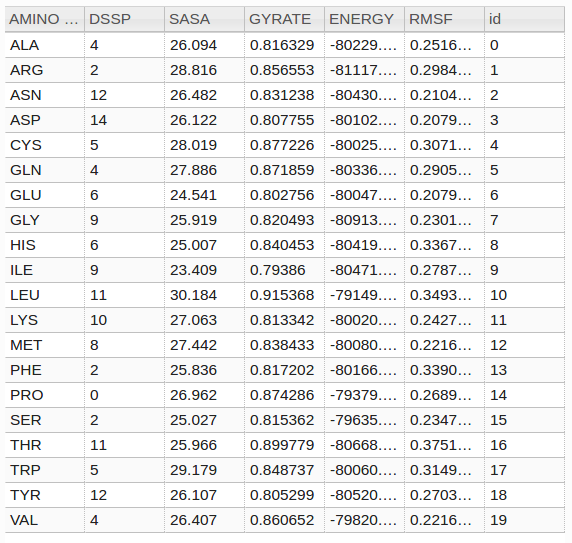
\includegraphics[width=0.8\linewidth]{figs/grid.png}
\caption{Overview of the used grid.} 
\label{fig:grid}
\end{figure}
\paragraph*{Item highlighting}
\paragraph*{Item selection}

\subsection{Parallel Coordinates}
\begin{figure}
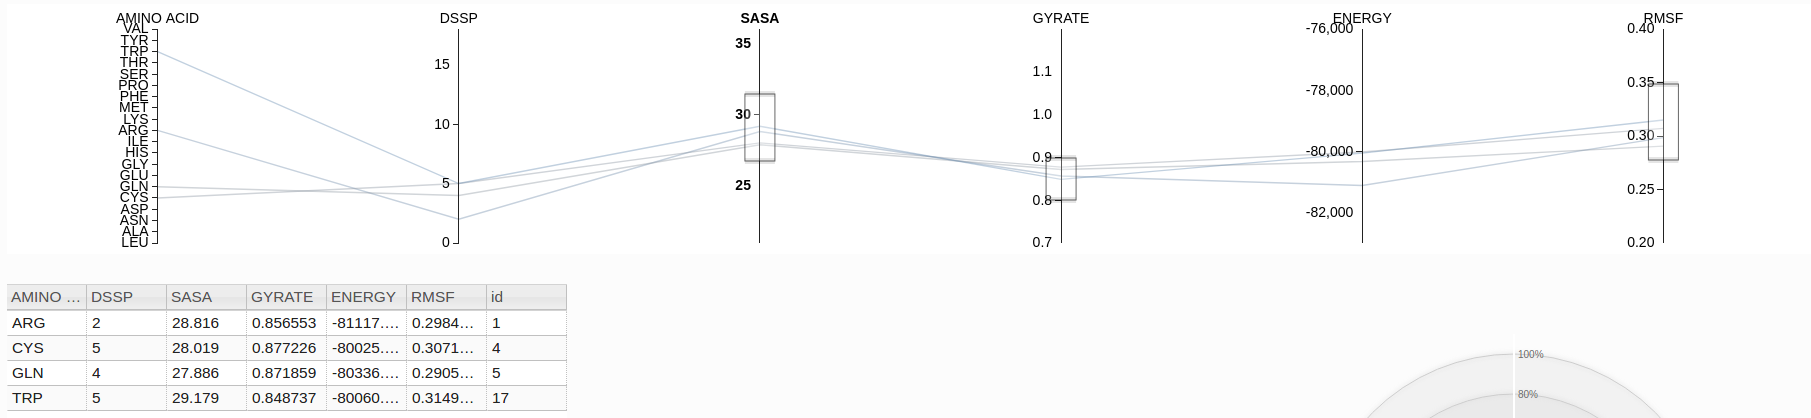
\includegraphics[width=0.8\linewidth]{figs/brush.png}
\caption{Example of the use of brush.} 
\label{fig:brush}
\end{figure}
\paragraph*{Axis brushing} Fig.~\ref{fig:brush}

\paragraph*{Axis sorting}
\paragraph*{Axis reordering}
\paragraph*{Recoloring by axis selection}

\subsection{Radar Plot}
\begin{figure}
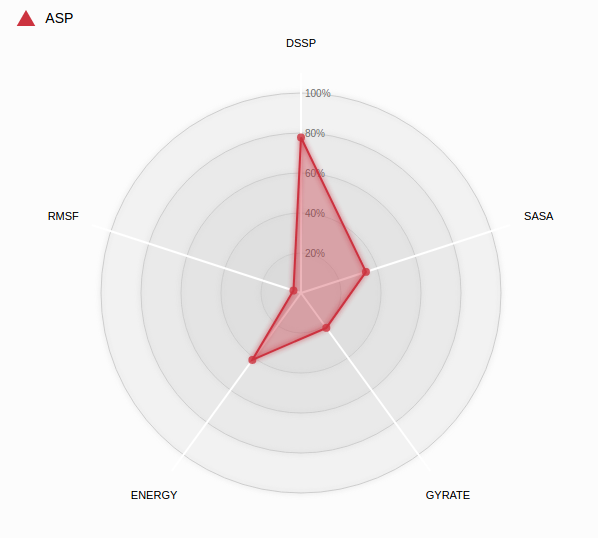
\includegraphics[width=0.8\linewidth]{figs/radar.png}
\caption{Example of one amino acid being visualized in the radar plot.} 
\label{fig:radar}
\end{figure}
\paragraph*{Item highlighting}

\subsection{Slider}

%==========================================
\section{Experiments}
%


%==========================================
\section{Results and Discussion}
%

%


%------------------------------------------------------------------------- 
\subsection{Future work}
%


%==========================================
\section{Conclusion}
%
A demo can be tested at: http://inf.ufrgs.br/~bigrisci/parallel-coordinates/examples/table.html


%==========================================
\iffinal
% use section* for acknowledgement
\section*{Acknowledgment}
%

\fi



%==========================================

% trigger a \newpage just before the given reference
% number - used to balance the columns on the last page
% adjust value as needed - may need to be readjusted if
% the document is modified later
%\IEEEtriggeratref{8}
% The "triggered" command can be changed if desired:
%\IEEEtriggercmd{\enlargethispage{-5in}}

\bibliographystyle{IEEEtran}
\bibliography{my}

\end{document}
